


\section{Auswertung}
\label{sec:auswertung}

In diesem Kapitel werden die aufgenommenen Messwerte ausgewertet.




\subsection{Schwingungsmoden und Bandbreite}
\label{sec:schwingungsmoden}

In diesem Abschnitt wurden drei aufeinanderfolgende Schwingungsmoden des Klystrons vermessen und graphisch dargestellt.
Ausserdem wurde die Bandbreite einer Mode vermessen und daraus die elektronische Bandbreite errechnet.
Die Messwerte zu den verschiedenen Reflektorspannungen sind in \autoref{tab:schwingmod} zu finden und wurden in vielfachem der maximal gemessenen Leistung angegeben, da ultimativ nur die Lage zueinander interessiert und es so leichter vergleichbar ist.


\begin{table}
\centering
\caption{Schwingungsmoden für verschiedene Reflektorspannungen}
\begin{tabular}{c c}
\toprule
{$V$[V]} & {$P/P_{\text{max}}$}\\
\midrule
220&	0,833\\
210	&0\\
230	&0\\
\midrule
140	&1\\
130	&0\\
150	&0\\
\midrule
80	&0,777\\
70	&0\\
90	&0\\
\bottomrule
\label{tab:schwingmod}
\end{tabular}
\end{table}



Zur graphischen Darstellung wurde für jede Mode eine Parabel an die Messwerte gefittet. Diese hat die Form:


\begin{equation}
P(V) = m\cdot (V - V_0)^2 + P_0
\label{eq:parabel}
\end{equation}

Die sich ergebenden Werte sind in \autoref{tab:schwingmod2} zu sehen. Für die Messwerte der Leistung wurde ein Fehler in der Größenordnung der letzten Nachkommastelle angenommen und dann genauso skaliert wie die Werte selbst ($P_{\text{Fehler}}/P_{\text{max}}$), um dimensionslos zu sein.

\begin{table}
\centering
\caption{Parameterwerte der Parabelfits}
\begin{tabular}{c c c}
\toprule
{$V_0$[V]} & {$P_0$} & {$m$[1/V]}\\
\midrule
{220,0000 \pm 0,2547}  & { 0,8330 \pm 0,0600} & {-0,0083 \pm 0,0007}\\
{140,0000 \pm 0,2121}  &  {1,0000 \pm 0,0600} & {-0,0100 \pm 0,0007}\\
{80,0000 \pm 0,2730}  &  {0,7770  \pm 0,0600} & {-0,0078 \pm 0,0007}\\
\bottomrule
\label{tab:schwingmod2}
\end{tabular}
\end{table}



Die Messwerte und sich ergebende Parabeln sind in \autoref{fig:schwingmod} dargstellt.

\begin{figure}
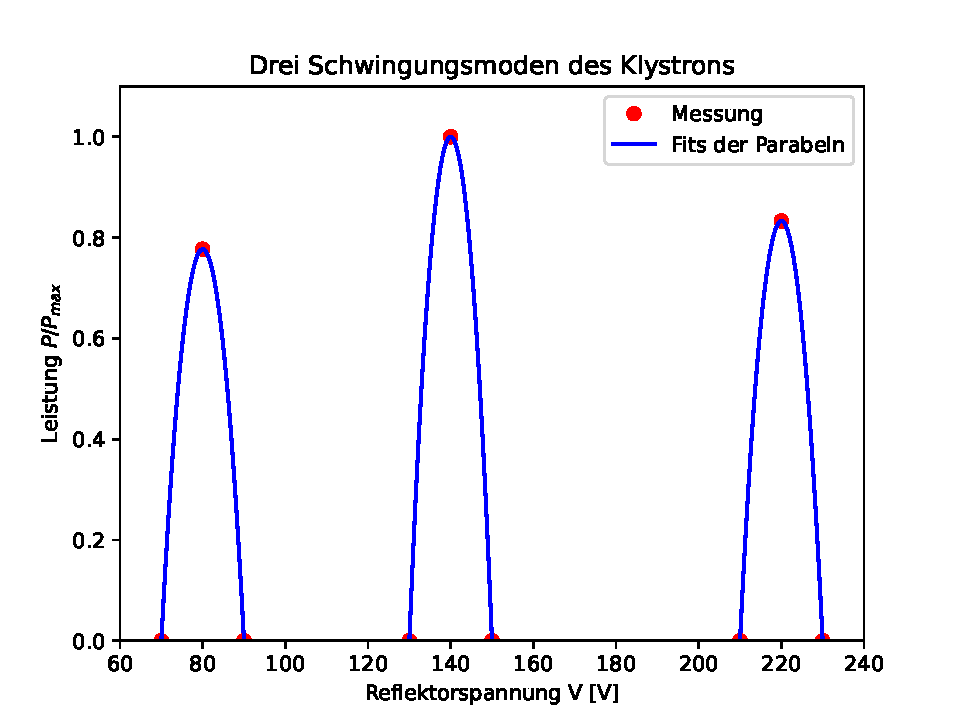
\includegraphics{figures/Schwingungsmoden.pdf}
\caption{Messwerte und Parabeln dreier Schwingungsmoden des Klystrons}
\label{fig:schwingmod}
\end{figure}


Die Messung zur Bandbreite einer Mode ist in \autoref{tab:bandbreite} zu finden. Für die Messwerte der Frequenz wurde eine Unsicherheit der Größe $0,5\,$MHz und für die Messwerte der Spannung eine Unsicherheit von $10\,$V angenommen.

\begin{table}
\centering
\caption{Messwerte zur Bestimmung der Bandbreite}
\begin{tabular}{c c}
\toprule
{$V$[V]} & {$f$[MHz]}\\
\midrule
220 & 9014\\
210&8999\\
230&9029\\
\bottomrule
\label{tab:bandbreite}
\end{tabular}
\end{table}


Die elektronische Bandbreite $B$ und Abstimmempfindlichkeit $E$ ergaben sich zu:

\begin{equation}
B = (30 \pm 0,707)\,\text{MHz}
\label{eq:bandbreite}
\end{equation}
\begin{equation}
E = (1,5 \pm 1,061) \frac{\text{MHz}}{\text{V}}
\label{eq:elbandbreite}
\end{equation}

Unsicherheiten wurden dabei mittels Gaußscher Fehlerfortpflanzung berechnet.

 







\subsection{Frequenz, Wellenlänge und Dämpfung}
\label{sec:fwd}


In diesem Abschnitt wird die Messung zur Bestimmung der Wellenlänge und der Frequenz der Mikrowellenstrahlung ausgewertet, sowie die, auf dem Dämpfungsglied angegebene Dämpfung, mit Messwerten verglichen.
Die gemessenen Positionen zweier aufeinanderfolgender Minima der stehenden Welle mit direkt gemessener Frequenz $f$ sind in \autoref{tab:minima} zu finden.


\begin{table}
\centering
\caption{Positionen zweier aufeinanderfolgender Minima}
\begin{tabular}{c c c}
\toprule
{$f$[MHz]} & {1. Minimum [mm]}&{2. Minimum [mm]}\\
\midrule
{$$9014\pm 0,5$$}&{$$62,6\pm 0,05$$}&{$$87,9\pm 0,05$$}\\
\bottomrule
\label{tab:minima}
\end{tabular}
\end{table}

Die Wellenlänge $\lambda_g$ ergibt sich aus dem doppelten des Abstands der Minima aus \autoref{tab:minima} zu:

\begin{equation}
\lambda_g = (50,6 \pm 0,141)\,\text{mm}
\label{eq:wellenlaenge}
\end{equation}

Alle Fehler in diesem Abschnitt wurden mittels Gaußscher Fehlerfortpflanzung ermittelt.
Die Frequenz $f$ lässt sich berechnen über folgende Formel:

\begin{equation}
f = c\cdot\sqrt{ (\frac{1}{\lambda_g})^2 + (\frac{1}{2a})^2 }
\label{eq:freq}
\end{equation}

Die Innenabmessung $a = (22,860 \pm 0,046)\,$mm des Hohlraumleiters und die Lichtgeschwindigkeit $c = 3\cdot 10^{11} \frac{\text{mm}}{\text{s}}$ wurden dabei der Versuchsanleitung entnommen.
Daraus ergibt sich die Frequenz zu:

\begin{equation}
f = (8843,47 \pm 14,79)\,\text{MHz}
\label{eq:freq2}
\end{equation}

Die Messwerte zur Dämpfung des Dämpfungsglied sind in \autoref{tab:daempf} zu sehen.


\begin{table}
\centering
\caption{Messwerte zur Dämpfung des Dämpfungsgliedes}
\begin{tabular}{c c c}
\toprule
{Mikrometereinstellung [mm]} & {gemessene Dämpfung [dB]} & {Dämpfung laut Eichkurve [dB]}\\
\midrule
3,00	&0	&16\\
3,18	&2	&19\\
3,31	&4	&20\\
3,59	&6	&24\\
3,70	&8	&25\\
3,89	&10	&29\\

\bottomrule
\label{tab:daempf}
\end{tabular}
\end{table}

Zur besseren Auswertbarkeit wurde danach die Dämpfungswerte aus der Eichkurve auf den ersten Messwert bezogen nach der Formel:

\begin{equation}
\text{Dämpfung}(x)_{\text{dB}} = x - 16\,\text{dB}
\label{eq:daempf}
\end{equation}

Die Dämpfungen in Abhängigkeit der Mikrometereinstellung sind in \autoref{fig:daempf} dargestellt.



\begin{figure}
\includegraphics{figures/Dämpfungsglied.pdf}
\caption{Gemessene und angegebene Dämpfungskurve}
\label{fig:daempf}
\end{figure}










\subsection{Stehwellenverhältnis}
\label{sec:welligkeit}


In diesem Abschnitt wird das Stehwellenverhältnis $S$, auch Welligkeit genannt, für verschiedene Sondentiefen und mit verschiedenen Messmethoden bestimmt.
Die direkte Messung der Welligkeit mittels des SWR-Meters für verschiedene Sondentiefen ist in \autoref{tab:swr} zu sehen.


\begin{table}
\centering
\caption{Direkt abgelesenes Stehwellenverhältnis $S$ am SWR-Meter}
\begin{tabular}{c c}
\toprule
{Sondentiefe [mm]} & {S}\\
\midrule
3&1,16\\
5&1,55\\
7&3,50\\
9&nicht ablesbar\\
\bottomrule
\label{tab:swr}
\end{tabular}
\end{table}


Die Messung zur 3\,dB-Methode ist in \autoref{tab:3db} zu finden. Die Werte $d_1$ und $d_2$ geben die Stellen an, an denen der Ausschlag des SWR-Meters um 3\,dB größer war als am dazu naheliegendsten Minimum. Der Abstand zweier aufeinanderfolgender Minima ist auch eingetragen, um daraus wie in \autoref{sec:fwd} die Wellenlänge $\lambda_g$ zu brechnen.



\begin{table}
\centering
\caption{SWR-Meter Einstellungen zur Bestimmung der Welligkeit mittels der 3\,dB Methode}
\begin{tabular}{c c c c}
\toprule
{$d_1$ [mm]} & {$d_2$ [mm]}& {1.Minimum [mm]}& {2. Minimum [mm]}\\
\midrule
91,20 & 89,50 & 103,00 & 78,90\\
\bottomrule
\label{tab:3db}
\end{tabular}
\end{table}

Das Stehwellenverhältnis lässt sich mittels folgender Formel berechnen:

\begin{equation}
S = \frac{\lambda_g}{\pi (d_1 - d_2)}
\label{eq:welligkeit1}
\end{equation}

Für die Unsicherheiten der Entfernungsmessung wurden $0,005$\,mm angenommen. Damit berechnet sich das Stehwellenverhältnis zu:

\begin{equation}
S = 9,025 \pm 0,038
\label{eq:welligkeit2}
\end{equation}

bei einer Sondentiefe von 9\,mm. Alle Unsicherheiten wurden in diesem Abschnitt mittels Gaußscher Fehlerfortpflanzung berechnet.\\
Die Messdaten für die Abschwächer-Methode sind in \autoref{tab:abschw} zu finden.


\begin{table}
\centering
\caption{Am Dämpfungsglied eingestellte Dämpfungen $A_1$ bzw $A_2$ zur Abschwächer-Methode}
\begin{tabular}{c c c c}
\toprule
{$A_1$ [dB]} & {$A_2$ [dB]}\\
\midrule
20 & 42\\
\bottomrule
\label{tab:abschw}
\end{tabular}
\end{table}

Das Stehwellenverhältnis lässt sich mit \autoref{eq:abschw} berechnen.

\begin{equation}
S = 10^{\frac{A_2 - A_1}{20}}
\label{eq:abschw}
\end{equation}

Es ergibt sich der Wert:

\begin{equation}
S = 12,589 \pm 2,0497
\label{eq:abschw2}
\end{equation}

Die Unsicherheit der Dämpfung wurde hierbei zu 1\,dB angenommen.





































